\chapter{Réalisation}

\section{Interface graphique}

\subsection{Panneaux et boutons}

Nos panneaux dérivent de la classe \emph{JPanel}, elle-même issue de la classe \emph{Panel}. Cette dernière fournit un composant Container permettant d'accueillir d'autres composants graphiques (sous-panneaux).\\

Le premier panneau (\textbf{panel1}) contient une zone de texte (\emph{JLabel}) afin d'afficher un message d'aide, ainsi qu'un menu déroulant (\emph{JComboBox}) pour le choix des algorithmes. \\

Le panneau central (\textbf{panel2}) est vide au lancement du plugin et son contenu varie en fonction de l'algorithme sélectionné. Par exemple pour l'algorithme Difference of Gaussian, les sous-panneaux sont créés dans la classe \texttt{panelDoG}. Pour cet algorithme, le \textbf{panel2} comprend :
\begin{itemize}
\item \textbf{infoPanel} contenant un \emph{JLabel} indiquant le type d'image requis.
\item \textbf{sigmaPanel} et \textbf{widthNoisePanel} qui contiennent des \emph{JLabel} et \emph{JTextField} afin de créer une zone dans laquelle peut entrer les paramètres nécessaires au déroulement du piquage. 
\item \textbf{debugCropPanel} quand à lui contient deux cases à cocher (\emph{JCheckBox}) pour activer ou non les modes de débogage et de crop. 
\end{itemize}
Les classes \texttt{panelImCorr} et \texttt{panelDilateDiff} servent à la création des sous panneaux des algorithmes Image Correlation et Dilate Difference respectivement. \\

Le dernier panneau (\textbf{panel3}) comporte quatre boutons (\emph{JButton}) devant répondre aux clics de la souris à l'aide d'un \emph{ActionListener}. \\

Enfin, le panneau principal (\textbf{mainPanel}) contient tous les panels cités précédemment. Sa taille détermine celle de la fenêtre du plugin. \\
Ces quatre panneaux sont crées dans la classe \texttt{PickFrame}, qui hérite de la classe \texttt{JFrame}. \texttt{PickFrame} peut également accéder à des méthodes de la classe \texttt{ActionListener}. \\

La figure suivante (Figure \ref{panneauxDetail}) donne un aperçu plus visuel de l'organisation de ces différents panneaux.
\begin{figure}[!ht] 
\begin{center}
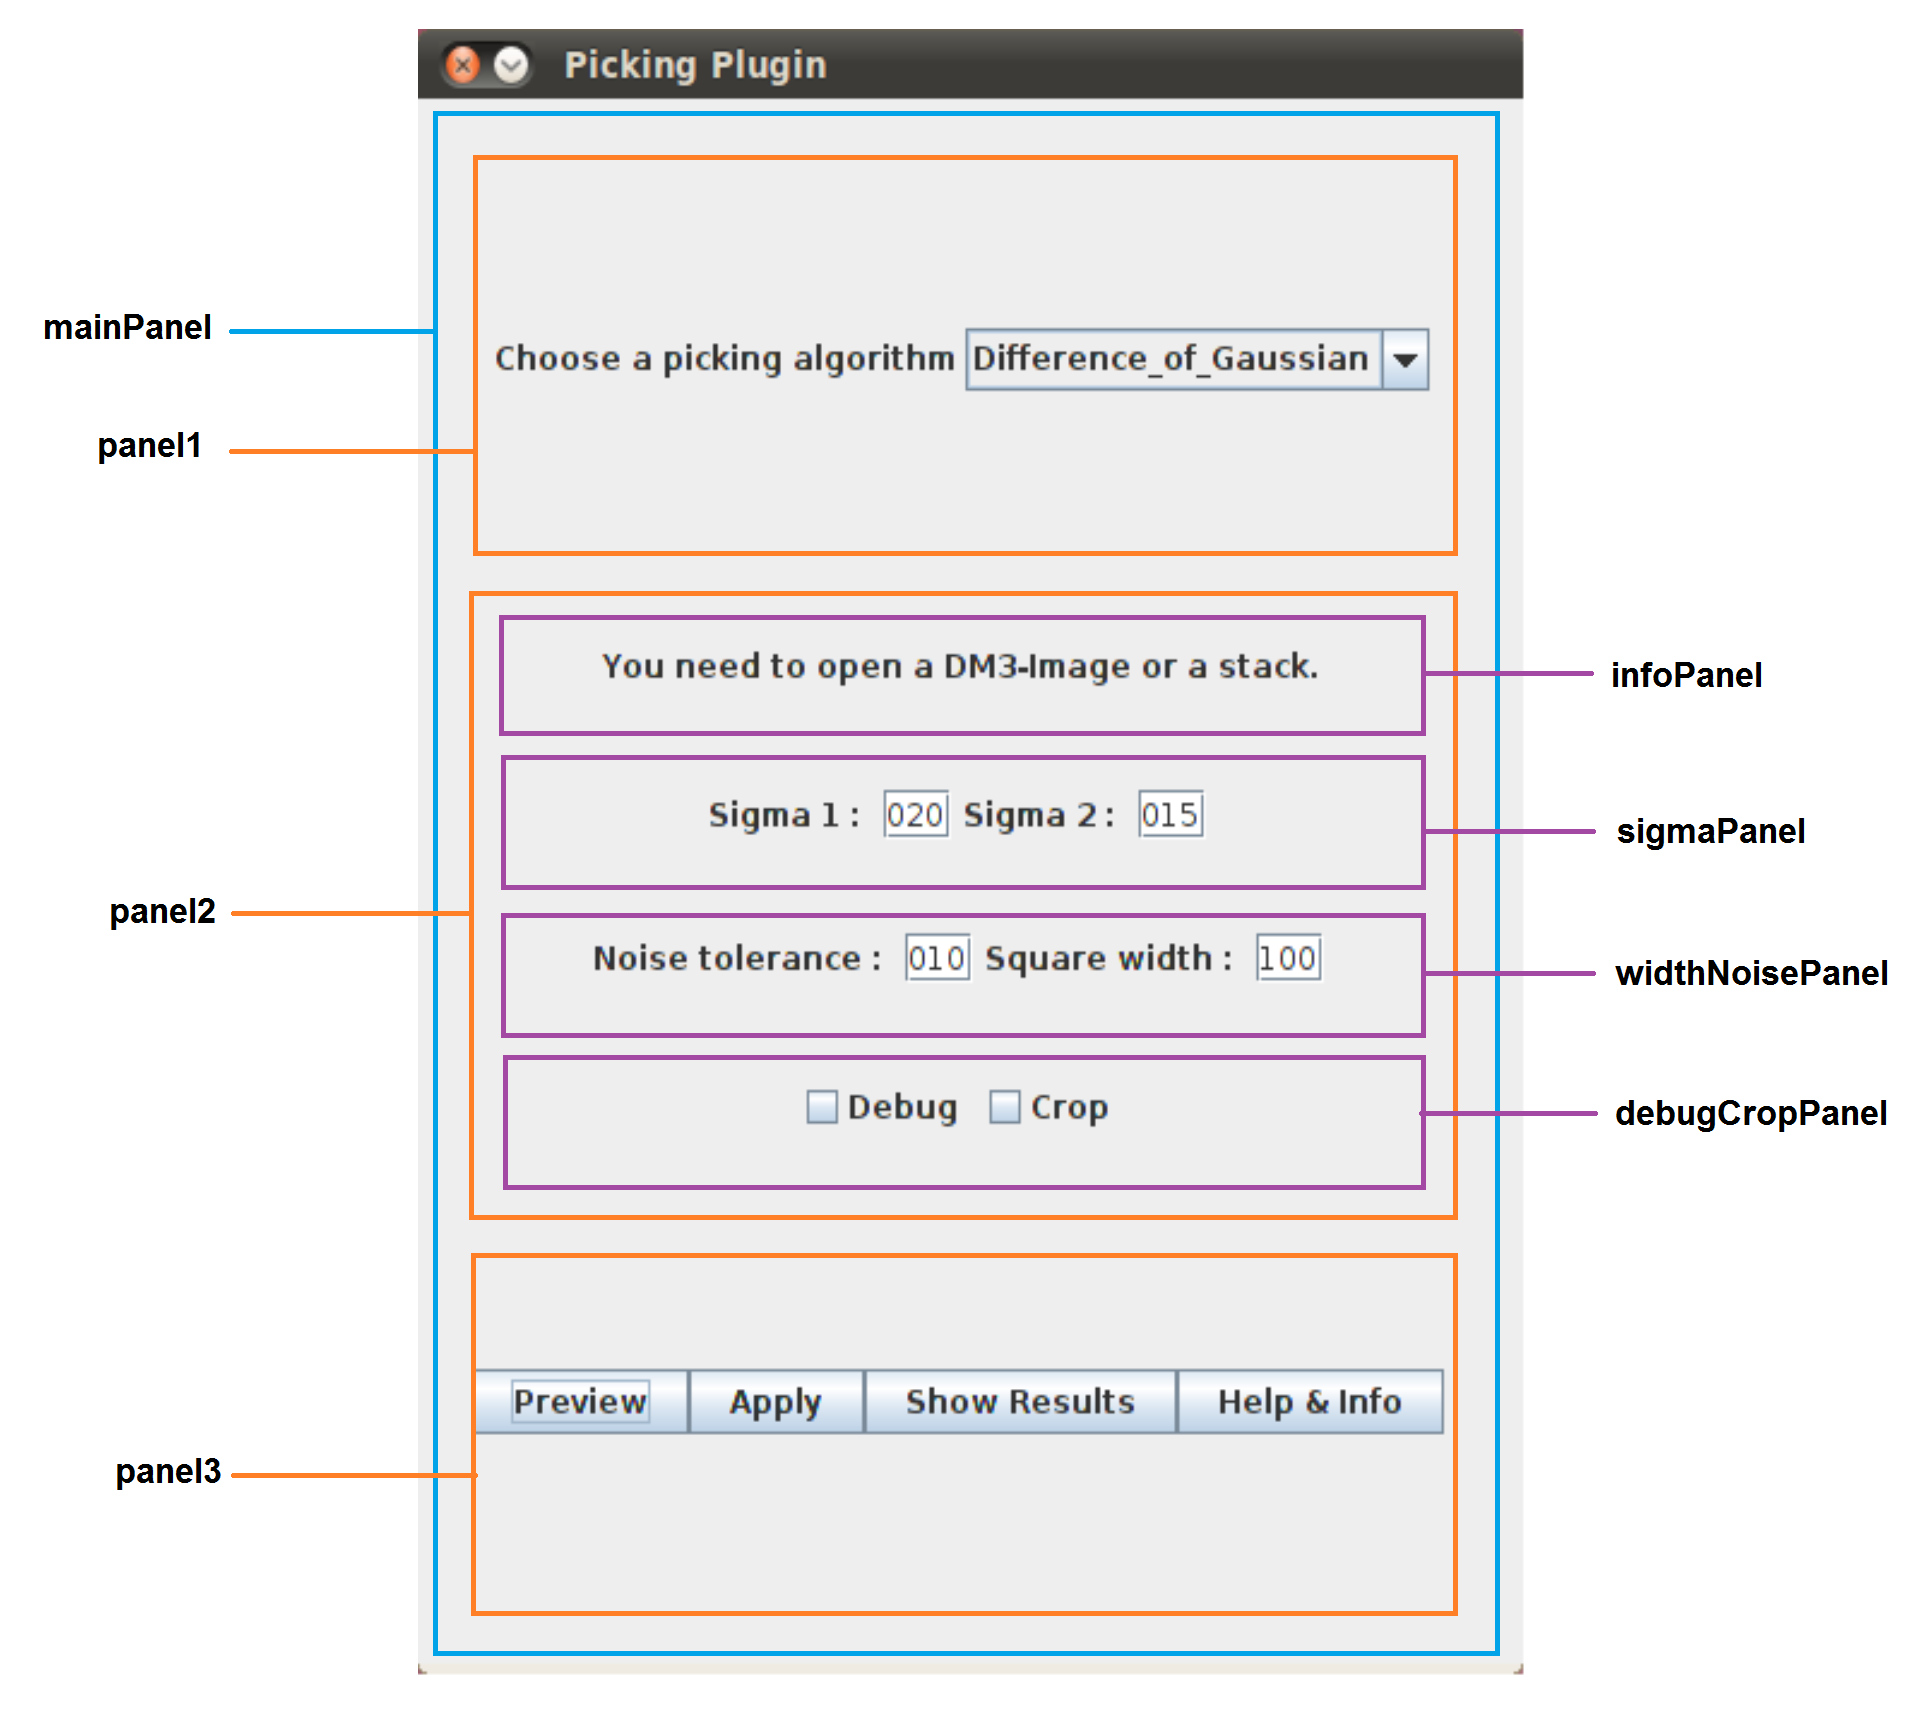
\includegraphics[width=0.8\textwidth]{plugin3-1.png}
\caption{Organisation des panels pour l'algorithme Difference of Gaussian}
\label{panneauxDetail}
\end{center}
\end{figure}
\pagebreak

\subsection{Affichage des résultats}

Lorsque l'utilisateur a coché la case "crop" avant de lancer la procédure de piquage, la classe \texttt{PickFrame} fait appel à la classe \texttt{Cropper} permettant de créer un stack. Les paramètres d'entrée de \texttt{Cropper()} sont une \emph{ImagePlus} (image courante du stack) et un tableau de doubles contenant les coordonnées des particules sélectionnées. \\
Lors de nos phases de tests, nous avons ajouté une autre fonction Cropper(), sans paramètres d'entrée. Nous y avons créé un tableau de coordonnées manuellement pour faciliter les essais. \\
A partir du tableau de doubles cité, la méthode \texttt{crop()} de \texttt{Cropper} fait appel à la méthode \texttt{setRoi()} d'\imj ~afin de retenir une zone carrée autour de la sélection. Cette zone va ensuite être dupliquée et ajoutée au stack sous la forme d'un \emph{ImageProcessor}. Ci-dessous un extrait de la méthode \texttt{crop()} :

\begin{small}
\begin{lstlisting}
if (z == currentSlice) {
  imp.setRoi(x, y, widthCrop, widthCrop);  
  // widthCrop = taille du carre de selection entree par l'utilisateur
  img2 = new Duplicator().run(imp);
  ImageProcessor ip2 = img2.getProcessor();
  ImageProcessor impTemp = ip2.resize(widthCrop,widthCrop);
  ims.addSlice(impTemp);
}
\end{lstlisting}
\end{small}	

Cette partie du code ne va s'exécuter que si le cadre de sélection de la particule ne dépasse pas le cadre de l'image de base. Les particules dépassant n'apparaitront pas dans le stack d'imagettes, mais on pourra retrouver leurs coordonnées dans le tableau de résultats final. \\

Par ailleurs, les résultats de la sélection peuvent être affichés sous la forme d'une \texttt{ResultsTable} si on clique sur le bouton "Show Results". Elle est construite grâce au tableau de doubles cité précédemment, qui est le paramètre d'entrée de la fonction \texttt{generate-} \texttt{CsvFile()}. 

\section{Récupération des paramètres}

Le singleton de la classe \texttt{Attributes} contient une table de hashage (\emph{HashTable}) dans laquelle sont stockés tous les paramètres entrés par l'utilisateur. Ces derniers sont accessibles grâce à des clés et donc réutilisables dans les algorithmes. La méthode  \texttt{synchronized()} dans la fonction \texttt{getInstance()} (voir ci-dessous) empêche toute instanciation multiple :

\begin{small}
\begin{lstlisting}
public final static Attributes getInstance() {
  if (Attributes.instance == null) {
    synchronized(Attributes.class) {
      if (Attributes.instance == null) {
        Attributes.instance = new Attributes();
      }
    }
  }
  return Attributes.instance;
}
\end{lstlisting}
\end{small}	

\section{Algorithmes}

Lorsque l'utilisateur fait le choix d'un algorithme de piquage parmi ceux qui lui sont proposés, cela fait appel à la classe \texttt{AlgoFactory} contenant plusieurs méthodes switch :
\begin{itemize}
\item \texttt{getPickPanel()} permet de récupérer le nom de l'algorithme choisi et d'afficher le panel2 correspondant.
\item \texttt{getPicker()} permet de lancer le piquage lorsque l'utilisateur appuie sur le bouton Apply.
\item \texttt{getPickerPreview()} permet de lancer le piquage lorsque l'utilisateur appuie sur le bouton Preview.
\end{itemize}

La présence d'un constructeur privé dans cette classe supprime le constructeur public par défaut. De plus, seul le singleton peut s'instancier lui même. \\

Une fois le panel2 chargé, l'appel aux procédures de piquage ne peut se faire que si l'on clique sur les boutons de prévisualisation (Preview) ou d'application à l'ensemble du stack (Apply). Les paramètres entrés par l'utilisateur sont sauvegardés dans la table de hashage grâce à la fonction \texttt{getInstance()} de la classe \texttt{Attributes}, puis récupérés, pour l'algorithme, par la fonction \texttt{setAttributes()} de la classe \texttt{PanelDoG} (pour suivre notre scénario). L'algorithme est ensuite appelé par la méthode \texttt{sliceSelection()} (Apply) ou par \texttt{picking()} (Preview). \\

La méthode \texttt{picking()} donne l'image courante du stack en paramètre de la méthode \texttt{pick()} alors que \texttt{sliceSelection()} parcourt le stack et appelle \texttt{pick()} autant de fois qu'il y a d'images dans le stack. \\

La méthode \texttt{pick()} quand à elle permet de lancer l'algorithme sur la sélection. Elle prend une ImagePlus et le numéro de l'image dans le stack en paramètres. Cette fonction récupère les paramètres entrés par l'utilisateur (grâce à \texttt{hashAttributes.get()}) et renvoie un tableau de résultats (X, Y, Slice). Voici un extrait du code de l'algorithme Difference of Gaussian :

\begin{small}
\begin{lstlisting}
Hashtable<String, String> hashAttributes = Attributes.getAttributes();
String sigma1 = hashAttributes.get("sig1");

imp.setSlice(currentslice);
ImagePlus imp1 = new Duplicator().run(imp);

String si1 = "sigma=" + sigma1;

imp1.setSlice(currentslice);
IJ.run(imp1, "Gaussian Blur...", si1);
\end{lstlisting}
\end{small}

Ici, nous obtenons le paramètre \textbf{sigma1} grâce à la table de hashage et la clé "\texttt{sig1}". Nous avons besoin de ce dernier pour appliquer le filtre gaussien sur l'image courante, c'est pourquoi nous le castons sous la forme d'un \emph{String}. Notons que la fonction \texttt{IJ.run()} permet de lancer une procédure \imj. \\
Nous avons choisi d'utiliser des vecteurs pour stocker les coordonnées ainsi que les numéros de slices car il nous est impossible de connaître à l'avance le nombre de particules qui vont être sélectionnées. \\
Nous avons fait en sorte de vider les tableaux de résultats entre le mode de prévisualisation et d'application, mais aussi entre deux applications ou deux prévisualisations. Ceci évite que les résultats ne s'ajoutent, ce qui fausserait la résultante du piquage. \\
Il en est de même pour tous les algorithmes. De plus, ceux-ci héritent de l'interface Picker. \\ 

VOIR POUR PICKER (interface ? ) \\

\section{Autres classes}

La classe \texttt{FFTMath} est issue de la classe \texttt{FFTMath} d'\imj, que nous avons modifié afin de pouvoir réaliser la corrélation d'images dans l'algorithme Image Correlation. \\

La classe \texttt{About} permet d'afficher les auteurs du plugin et le moyen de nous contacter si besoin. \\

La classe \texttt{InfoHelp} affiche une aide sur le fonctionnement du plugin si l'utilisateur  clique sur le bouton "Hepl \& Info". 


\section{Applications}

Le résultat affiché sur l'image correspond aux positions des particules sur l'image courante, ou la dernière image dans le cas d'un stack.
L'utilisateur peut choisir d'afficher un tableau contenant les coordonnées (abscisses, ordonnées et positions dans le stack) des particules sélectionnées et pourra le sauvegarder. \\
De plus, s'il le désire, un stack contenant les particules sélectionnées aux positions obtenus est créé (éliminant les particules trop près du bord de l'image) et affiché.

\begin{figure}[!ht]
\begin{center}
 \begin{minipage}{.450\linewidth}
  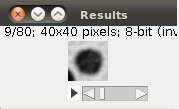
\includegraphics[width=0.75\textwidth]{cropblob.png}  
 % \caption{Difference de Gaussienne (blobs)}
 \end{minipage} \hfill
\begin{minipage}{.450\linewidth}
  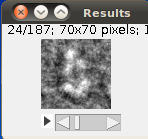
\includegraphics[width=0.5\textwidth]{cropprotDog.png}   
  %\caption{Difference de Gaussienne (protéines)}
 \end{minipage} \hfill
\caption{Exemple d'images formant le stack de particules (blobs et protéines)}
\end{center}
\end{figure}

\subsubsection*{Statistiques}

La Différence gaussienne permet d'obtenir les résultats suivants :

\begin{figure}[!ht]
\begin{center}
 \begin{minipage}{.450\linewidth}
  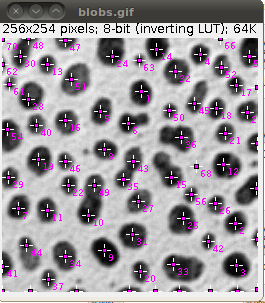
\includegraphics[width=0.75\textwidth]{blobsDog.png}  
 % \caption{Difference de Gaussienne (blobs)}
 \end{minipage} \hfill
\begin{minipage}{.450\linewidth}
  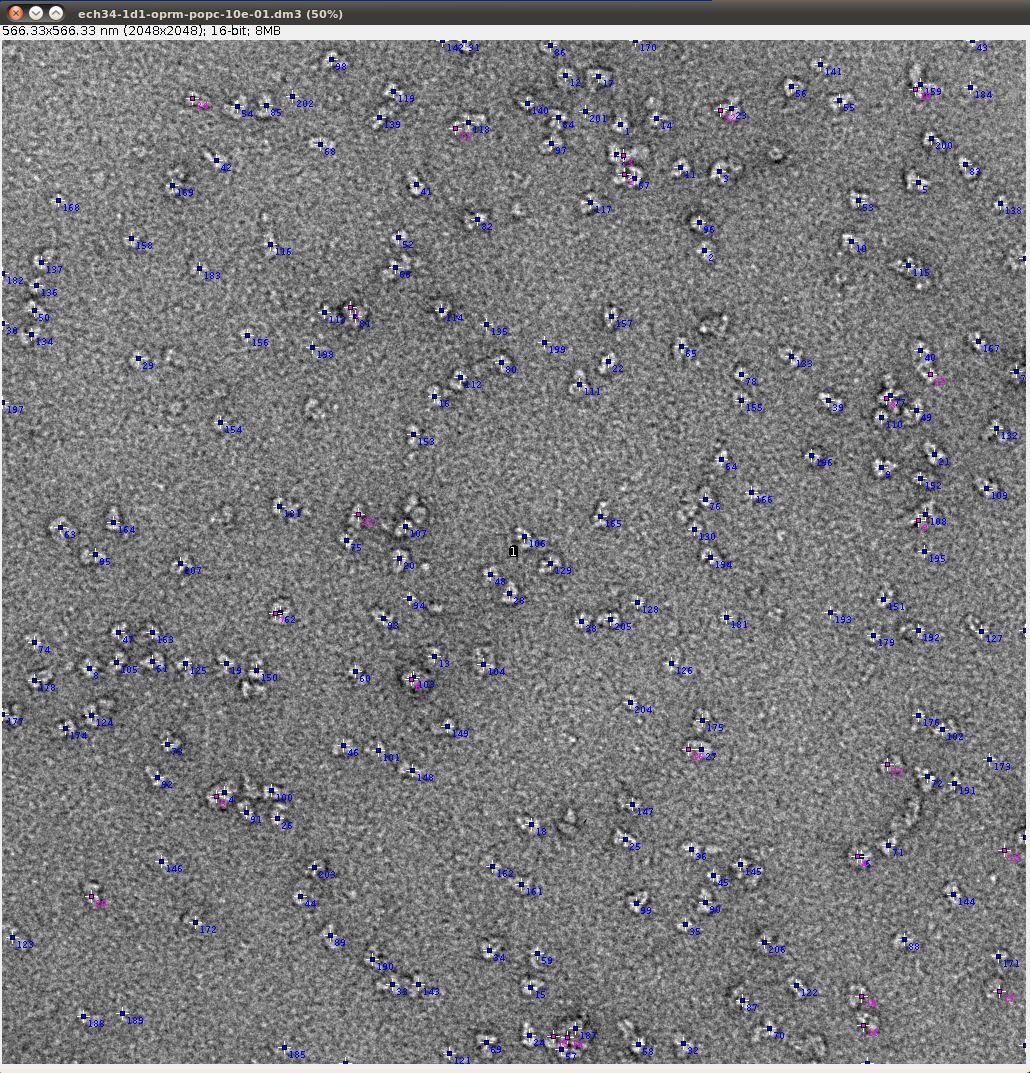
\includegraphics[width=1\textwidth]{protDog.png}   
  %\caption{Difference de Gaussienne (protéines)}
 \end{minipage} \hfill
\caption{Différence Gaussienne (blobs et protéines)}
\end{center}
\end{figure}

La Différence de dilatation permet d'obtenir les résultats suivants :






























